% ===========================================
% Template for ICMC 2017 (version2)
% adapted from earlier LaTeX paper templates for the ICMC, SMC, etc...
% ===========================================

\documentclass{article}
\usepackage{icmc2017template}
\usepackage[utf8]{inputenc}
\usepackage{times}
\usepackage{ifpdf}
\usepackage{soul}
\usepackage[english]{babel}
%\usepackage{cite}

\usepackage{enumitem}
%\usepackage{graphicx}
\usepackage{balance}
%\usepackage{hyperref}
\usepackage{amssymb,amsmath} 
\usepackage{verbatim}
\usepackage{color}
\usepackage{float}

% ====================================================
% ====================================================
\definecolor{mygrey}{gray}{0.95}

\newcommand{\OSC}[1]	{{\fontsize{8.5pt}{8pt} \selectfont\texttt{#1}}}
\newcommand{\note}[1]	{\textcolor{red}{(#1)}}

\newcommand{\lowTilde}{\texttildelow}
\newcommand{\tab}{\hspace*{4mm}}
\let\olditemize\itemize
\let\oldenditemize\enditemize
\renewenvironment{itemize} 	{\olditemize \renewcommand{\labelitemi}{$\bullet$} \setlength{\itemsep}{0mm}}{\oldenditemize}

\newcommand{\sample}[1]		{\vspace{-0.2em}\begin{center}\colorbox{mygrey}{\begin{minipage}[t]{0.98\columnwidth} {\small \texttt{#1}}\end{minipage}}\end{center}}
% ====================================================
% ====================================================



%%%%%%%%%%%%%%%%%%%%%%%% Some useful packages %%%%%%%%%%%%%%%%%%%%%%%%%%%%%%%
%%%%%%%%%%%%%%%%%%%%%%%% See related documentation %%%%%%%%%%%%%%%%%%%%%%%%%%
%\usepackage{amsmath} % popular packages from Am. Math. Soc. Please use the 
%\usepackage{amssymb} % related math environments (split, subequation, cases,
%\usepackage{amsfonts}% multline, etc.)
%\usepackage{bm}      % Bold Math package, defines the command \bf{}
%\usepackage{paralist}% extended list environments
%%subfig.sty is the modern replacement for subfigure.sty. However, subfig.sty 
%%requires and automatically loads caption.sty which overrides class handling 
%%of captions. To prevent this problem, preload caption.sty with caption=false 
%\usepackage[caption=false]{caption}
%\usepackage[font=footnotesize]{subfig}

% ====================================================
% ================ Define title and author names here ===============
% ====================================================
%user defined variables
\def\papertitle{INScore Time Model}
\def\firstauthor{D. Fober \quad Y. Orlarey \quad S. Letz}
\def\secondauthor{Second Author}
\def\thirdauthor{Third Author}
\def\fourthauthor{Fourth Author}
\def\fifthauthor{Fifth Author}
\def\sixthauthor{Sixth Author}

% adds the automatic
% Saves a lot of output space in PDF... after conversion with the distiller
% Delete if you cannot get PS fonts working on your system.

% pdf-tex settings: detect automatically if run by latex or pdflatex
\newif\ifpdf
\ifx\pdfoutput\relax
\else
   \ifcase\pdfoutput
      \pdffalse
   \else
      \pdftrue
  \fi
\fi

\ifpdf % compiling with pdflatex
  \usepackage[pdftex,
    pdftitle={\papertitle},
    pdfauthor={\firstauthor, \secondauthor, \thirdauthor},
    bookmarksnumbered, % use section numbers with bookmarks
    pdfstartview=XYZ % start with zoom=100% instead of full screen; 
                     % especially useful if working with a big screen :-)
   ]{hyperref}
  %\pdfcompresslevel=9

  \usepackage[pdftex]{graphicx}
  % declare the path(s) where your graphic files are and their extensions so 
  %you won't have to specify these with every instance of \includegraphics
  \graphicspath{{./figures/}}
  \DeclareGraphicsExtensions{.pdf,.jpeg,.png}

  \usepackage[figure,table]{hypcap}

\else % compiling with latex
  \usepackage[dvips,
    bookmarksnumbered, % use section numbers with bookmarks
    pdfstartview=XYZ % start with zoom=100% instead of full screen
  ]{hyperref}  % hyperrefs are active in the pdf file after conversion

  \usepackage[dvips]{epsfig,graphicx}
  % declare the path(s) where your graphic files are and their extensions so 
  %you won't have to specify these with every instance of \includegraphics
  \graphicspath{{./figures/}}
  \DeclareGraphicsExtensions{.eps}

  \usepackage[figure,table]{hypcap}
\fi

%setup the hyperref package - make the links black without a surrounding frame
\hypersetup{
    colorlinks,%
    citecolor=black,%
    filecolor=black,%
    linkcolor=black,%
    urlcolor=black
}


% ====================================================
% ================ Title and author info starts here ===============
% ====================================================
% Title.
% ------
\title{\papertitle}

% Authors
% Please note that submissions are anonymous, therefore 
% authors' names should not be VISIBLE in your paper submission.
% They should only be included in the camera-ready version of accepted papers.
% uncomment and use the appropriate section (1, 2 or 3 authors)
%
% Single address
% To use with only one author or several with the same address
% ---------------
\oneauthor
   {\firstauthor} {Grame \\
  Centre nationale de création musicale \\
  Lyon - France \\
     {\tt {\small \{fober, orlarey, letz\}@grame.fr}}}


% ====================================================
% =============== The document content starts here ===============
% ====================================================
\begin{document}
%
\capstartfalse
\maketitle
\capstarttrue
%
\begin{abstract}
INScore is an environment for augmented interactive music score design turned towards unconventional uses of music notation, without excluding conventional approaches. In this environment, although all the objects of a score have a temporal dimension, the time remains \emph{fixed} i.e. the date (or duration) of an object does not change, except on message reception (sent from an external application or resulting from events handling). Thus, INScore does not include a time manager in the classic sense of the term.
This choice was based on the fact that the system was originally designed for uses coupled with sound production software (e.g. Max/MSP, Pure Data), that have more strict real-time constraints than INScore's graphical environment.
However, the need to introduce dynamic time has gradually emerged, leading to an original model, both \emph{continuous} and  \emph{event based}. The paper presents this model and its properties in the environment of INScore.
\end{abstract}
%


%==============================================================
\section{Introduction}\label{sec:introduction}
Time manipulations in the environments for musical composition can be expressed in very different ways.

In OpenMusic, there are three main types of time expression: "musical time (i.e. time of symbolic notation, relative to a tempo), proportional time (expressed in milliseconds) and continuous time (defined by mathematical functions)"~\cite{bresson08}.

In other environments such as Antescofo \cite{acont08} or iScore \cite{AllombertDA08}, time is also \textit{event based} and can be described in terms of Allen relations \cite{Allen:1983:MKT:182.358434}, which allows to introduce reactive aspects in the musical pieces.
More recently, these reactive aspects have also been introduced in OpenMusic \cite{bresson:hal-00965747}, testifying to their importance in contemporary compositional approaches.

Time in INScore \cite{Fober:12a} is \emph{static}: all objects have a date and duration expressed in musical time that are fixed by the score description. The common temporal dimension of all objects of a score allows to represent their temporal relations in the graphical space \cite{fober:10b}. The \emph{animation} of the time (i.e. the modification of the temporal attributes of an object) occurs on OSC messages receipt. These messages are necessarily transmitted from an external application.

The choice of a \emph{static} time was due to a design originally turned to uses coupled with sound production software (e.g. Max/MSP, Pure Data), that have strict real-time constraints and offer effective and accurate time management mechanisms. Nevertheless, the reactive aspects were quickly taken into account with the introduction of \textit{events}, which allow to interact with the music score \cite{Fober:13b}. Initially, the typology of these events includes classical user interactions events (e.g. mouse events), and introduces events in the temporal domain (notably time intervals monitoring). This mechanism of \textit{events} paved the way for an original approach to music score programming by providing the user with the ability to place messages - and thus interactions - in the temporal space. Nevertheless, as time was always \emph{static}, the use of an external application remained necessary to actuate it.

The need for a \emph{dynamic} time has thus emerged. It has been solved in a simple way, with the introduction of an additional attribute to the objects of a score: the \emph{tempo}. This simple addition, however, has an important impact on the design of the time in INScore and on the dynamic aspects of the score. We will first present the musical time model, which is controlled by the tempo. We will then see how this time combines with event-based time, and allows to program \emph{autonomous} dynamic scores. We will finally show some use cases before concluding and giving some perspectives for the extension of the temporal dimensions of the objects of a score.


%==============================================================
\section{The musical time model}\label{mustime}

From the user point of view and for a given object, time is active when its tempo attribute is non-zero: a non-zero tempo value moves the object in musical time, according to its tempo and the flow of absolute time. \\
We will talk about \emph{date} to refer to the musical time of an object, and about \emph{time} to refer to a point in the flow of absolute time. \\

Let $t_0$ be the time of activation of an object time and $v$ the value of its tempo, the date $d_t$ of the object at a time $t$ is given by a time function $f$ Such that:
\begin{equation}
%\[
	 f(t) \to d_t = d_t{_0} + (t - t_0) \times v \times k , \quad t \geqq t_0
%\]
\label{timeeq}
\end{equation}
where $d_i$ is the date of the object at time $t_i$ and $k$ a constant to convert absolute time to musical time. In practice, the absolute time is expressed in milliseconds and the unit of musical time is the whole note. Therefore, the value of the constant $k$ is $1/1000 \times 60 \times 4$.

Each object of a score has an independent tempo. The tempo value is signed, meaning that an object can move in any direction of time (forward or backward). There are few environments allowing to express this reversal of time in a simple and natural way, we can quote IanniX \cite{coduys04}, a graphical sequencer inspired by the work of Iannis Xenakis and that can viewed as a \emph{time writing system}.


%=======================================
\subsection{Implementation}

In INScore, the time granularity is that of the display: the system runs asynchronously and a periodic time task processes the incoming messages and computes the graphical rendering. In practice, since the effects of time are visible only in the graphical space, we consider that it isn't necessary to adopt a finer time resolution.

In the other hand, the frequency of the time task can be variable:
\begin{itemize}
\item by default, it is performed every 10 ms but the user can freely change this value by sending the \OSC{rate} message to the application, followed by a value in milliseconds.
\item the time task is not reentrant and the complexity of the display can potentially slow it down.
\end{itemize}
Thus, and at each time task, the system measures the time actually elapsed. Then, objects whose tempo is non-zero use this value to compute an offset expressed in musical time as indicated in (\ref{timeeq}), then self-send a \OSC{ddate} message (moving the date in relative mode) with the corresponding value.

\begin{figure}[h]
   \centering
   \sample{/ITL/scene/obj tempo 60 \\
   \\
-> /ITL/scene/obj ddate $f(r_i)$ \\
-> /ITL/scene/obj ddate $f(r_{i+1})$ \\
-> /ITL/scene/obj ddate $f(r_{i+2})$ \\
-> ...
}
   \caption{A sequence of messages that activate the time of an object \OSC{obj}. Messages prefixed by \OSC{->} are generated by the object itself. $r_{i}$ is the time elapsed between task $i$ and $i-1$.}
   \label{fig:tempo}
\end{figure}

To be consistent with the overall system, this implementation is entirely message-based. Thus it is compatible with all INScore mechanisms, such as the message \emph{forwarding} system.

%==============================================================
\section{The events-based time.}\label{evtime}

The \emph{events-based} approach of time in INScore preceded the musical time model and was first presented in \cite{fober13b}. As a reminder, the process of event interaction relies on the association of messages with events of the system. These messages are sent when the event they are associated with occurs. The general message format for creating such associations is described in figure \ref{fig:watch}.

\begin{figure}[htbp]
\centerline{
	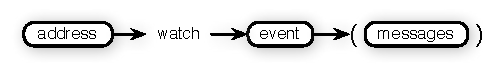
\includegraphics[width=0.95\columnwidth]{imgs/watch}}
\caption{Format of an interaction message : the \OSC{watch} method installs a list of messages associated to the event\OSC{event}.}
\label{fig:watch}
\end{figure}

With the first version presented, the event's typology was limited to classical UI events (such as mouse clicks), extended in the time domain (see table \ref{tbl:evts}). 

\begin{table}[htp]
\begin{center}
\begin{tabular}{c|c}
Graphic domain & Time domain \\
\hline
mouseDown 		& timeEnter	\\
mouseUp			& timeLeave	\\
mouseEnter		& durEnter		\\
mouseLeave		& durLeave		\\
mouseMove		&				\\
\end{tabular}
\end{center}
\caption{Main events of the system in its initial version.}
\label{tbl:evts}
\end{table}%

This typology has been significantly extended to include:
\begin{itemize}
\item any attribute of an object: the modification of an attribute value may generate the corresponding event, that carries the name of the attribute (e.g. \OSC{x, y date}, etc. .).
\item the intrinsic data of an object, i.e. those defined by a \OSC{set} message. That's the \OSC{newData} event, introduced for the purpose of symbolic scores composition \cite{Lepetit-Aimon_tenor2016}.
\item arbitrary events defined by the user.
\end{itemize}

Any event can be triggered by sending an \OSC{event} message followed by its parameters. Conceptually, this message  is equivalent to calling a parameterized function that generates OSC messages as output.
This logic is particularly consistent for user events, which can take a variable number of parameters, that are then available to the associated messages under the form of variables named $\$1 ... \$n$. Figure \ref{fig:uevent} shows a 2-arguments user event example.

\begin{figure}[h]
   \centering
   \sample{/ITL/scene/obj watch MYEVENT ( \\
\tab/ITL/scene/t1 set txt \$1, \\
\tab/ITL/scene/t2 set txt \$2 \\
);   \\   
/ITL/scene/obj event MYEVENT \\
\hspace*{25mm}"This text is for t1"\\
\hspace*{25mm}"This one is for t2"; 
}
   \caption{Definition of a user event named \OSC{MYEVENT} that expects 2 parameters referenced by \$1 and \$2. This event is then triggered with 2 strings as arguments.}
   \label{fig:uevent}
\end{figure}

The temporal dimension of this \emph{event-based} logic allows to place \emph{functions} in the time space, under the form of events that activate messages, which can modify the state of the system and/or be addressed to external applications using INScore extended OSC addressing scheme. Figure \ref{fig:events} gives an example.
  
\begin{figure}[h]
   \centering
   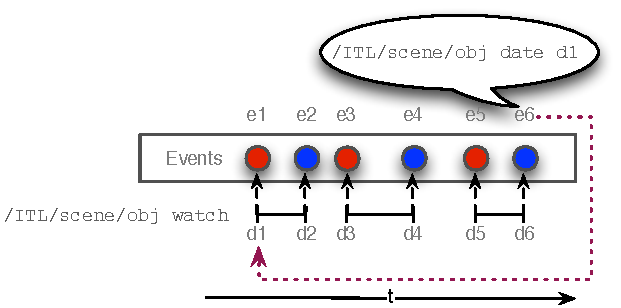
\includegraphics[width=0.95\columnwidth]{imgs/events}
   \caption{Example of events placed in the time space for an object \OSC{obj}. These events are associated with time intervals (\OSC{timeEnter} and \OSC{timeLeave}) and are triggered when entering (red) or leaving (blue) these intervals. The last event (\OSC{e6}), sends a \OSC{date} message that creates a loop by positionning the object at the beginning of the first interval.}
   \label{fig:events}
\end{figure}


%==============================================================
\subsection{Implementation}

Each object of a score handles relationships between a set of events $\mathbb{E}$ and a set of messages $\mathbb{M}$. The set of events $\mathbb{E}_o$ of an object $o$ is a polymorphic set defined as:
\[
	\mathbb{E}_o = \mathbb{A}_o \cup \mathbb{U}_o \cup \mathbb{T}_o \cup \mathbb{T'}_o \cup \mathbb{K}  
\] 
where:
\begin{itemize}
\item[-] $\mathbb{A}_o$ is the set of the object attributes, 
\item[-] $\mathbb{U}_o$ is the set of the object user defined events, 
\item[-] $\mathbb{T}_o$ and $\mathbb{T'}_o$ are respectively the set of time intervals monitored at input and at output,
\item[-] $\mathbb{K}$ is the set of UI events (\OSC{mousexxx, touchxxx}).
\end{itemize}

An event $e$ will be called a trigger when:
\[
	\exists (e, m) \in \mathbb{E}_o \times \mathbb{M}_o  
\] 
The messages from $m$ are then sent.

Computation of an event $e$ depends on the event type:
\begin{itemize}
\item[-] for a message $x$ addressed to an object $o$, an event will be triggered if $x \in \mathbb{A}_o$, 
\item[-] for a message \OSC{event} $x$ addressed to an object $o$, an event will be triggered if $x \in \mathbb{U}_o \cup \mathbb{A}_o \cup  \mathbb{K}$,
\item[-] for a message \OSC{date} $x$ addressed to an object $o$ that has the date $d$, an event will be triggered if:\\ 
\hspace*{3.5mm} $\exists i \in \mathbb{T}_o\ \ |\ (x \in i\ \land\ d \not\in i)$ \\
or $\exists i \in \mathbb{T'}_o\ |\ (x \not \in i\ \land\ d \in i)$,
\item[-] events from $\mathbb{K}$ are computed by the host system.
\end{itemize}

%==============================================================
\section{Dynamic music scores}

The combination of musical and event time allows to design autonomous dynamic scores. In the following example, 3 objects \OSC{o1, o2} and \OSC{o3} activate each other (figure~\ref{fig:ex1}) according to the time diagram described in figure~\ref{fig:sample}. It makes use of the 2 \emph{user} events \OSC{START} and \OSC{STOP}, that are described in figure \ref{fig:ex2}.

\begin{figure}[h]
   \centering
\sample{/ITL/scene/o1 watch timeLeave 0 \$t2 \\
   \tab( /ITL/scene/o2 event START );\\
	/ITL/scene/o1 watch timeLeave 0 \$d1 \\
	\tab( /ITL/scene/o1 event STOP );\\
	/ITL/scene/o2 watch timeLeave 0 \$d2 \\
	\tab( /ITL/scene/o2 event STOP, \\
	\tab \tab/ITL/scene/o3 event START );\\
	/ITL/scene/o3 watch timeLeave 0 \$d3 \\
	\tab( /ITL/scene/o3 event STOP, \\
	\tab \tab/ITL/scene/o1 event START );
}
   \caption{Mutual activationof 3 objects \OSC{o1, o2, o3} according to a predefined time scheme.}
   \label{fig:ex1}
\end{figure}

The variables \OSC{\$t1, \$d1, \$d2} and \OSC{\$d3} are instantiated with values corresponding to the figure \ref{fig:sample}. Note that the object \OSC{o3} loops the system by triggering the \OSC{START} event of the object \OSC{o1}.

\begin{figure}[h]
   \centering
\sample{/ITL/scene/o* watch STOP ( \\
   \tab/ITL/scene/\$self tempo 0,\\
   \tab/ITL/scene/\$self alpha \$alpha	\\
);\\
\\
/ITL/scene/o* watch START ( \\
   \tab/ITL/scene/\$self tempo 120,\\
   \tab/ITL/scene/\$self alpha 255,\\
   \tab/ITL/scene/\$self date 0\\
);
}
   \caption{Definition of the user events \OSC{START} and \OSC{STOP}.}
   \label{fig:ex2}
\end{figure}

The \OSC{START} and \OSC{STOP} events respectively activate and deactivate the receiver object time by changing the value of its tempo and modifying its graphical appearance (alpha channel) to account for the activation of time. The \OSC{START} event also sets the date of the object to 0, which allows looping the system by \OSC{o3}.
\begin{figure}[h]
   \centering
   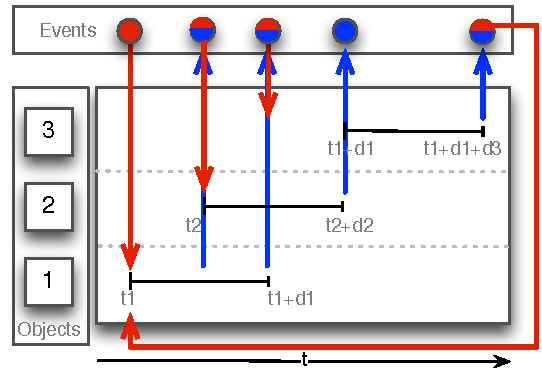
\includegraphics[width=0.8\columnwidth]{imgs/sample}
   \caption{Representation of the time activation for 3 objects of the score. The red color is used for \OSC{START} events, blue for \OSC{STOP}}
   \label{fig:sample}
\end{figure}


%==============================================================
\subsection{Jeu est un autre}

\emph{Jeu est un autre} from Vincent Carinola is a pedagogical music piece for computer and a variable number of performers, where Max/MSP is used to compute sound processes and to activate a dynamic music score intended to performers. 

The music score (figure \ref{fig:sample}) consists of a set of graphics with labels (sculpture, zebra, pace, texture, turn) connected by \emph{paths}. Each graphic (that we will call \emph{stations}) is associated to an instrumental play mode and to specific sound processes, based on materials prepared by the students. For example, the path \emph{whisper} indicates that \emph{the passage from one graphic to another is done by crossing a path inhabited by whispers. It is necessary to find here, in the instrumental and vocal play, what would be most like a story that would be told very softly, whispering.}\footnote{excerpt from the instructions given with the score}

In a given way, the computer plays the role of conductor: it computes sound sequences based on pre-recorded materials and activates \emph{paths} or \emph{stations} for variable durations, dynamically computed. The \emph{paths} and possible \emph{stations} are indicated in the figure \ref{fig:sample} by the labels P1 to P13.

The dynamic aspects of the score are defined with user events that carry the name of the corresponding labels. These events take a duration as parameter, so that the following message is enough to activate a \emph{path} or a \emph{station}:\\
\tab \tab \OSC{/ITL/scene Px d} \\
where \OSC{Px} is the user event name (\OSC{P1...P13})\\
 and \OSC{d} the corresponding duration. 
 
Thus, it's a high-level approach that allows to \emph{conduct} the score in real time from Max/MSP side.

Visually, the score accounts for these events in the graphic space in two ways:
\begin{itemize}
\item for \emph{stations} (events \ OSC {P1 ... P4} and \ OSC {P13}): using the alpha channel of the corresponding graphic to indicate its activation.
\item for \emph{paths} (events \ OSC {P5 ... P12}): by moving a cursor along the path, in the corresponding direction.
\end{itemize}

Schematically, the implementation of these events relies on an object named \OSC{cursor} that moves in time at a given tempo, depending on a time unit fixed by convention.

Activation of a \emph{stations} consists in changing the alpha channel of the corresponding graphic, activating the cursor time and instantiating an event for the end of the duration computed by Max/MSP (figure \ref{fig:station}).
\begin{figure}[h]
   \centering
\sample{/ITL/scene watch P1 ( \\
\tab/ITL/scene/g1 alpha 255, \\
\tab/ITL/scene event STATION \$tempo '\$1' \\
); \\
\\
/ITL/scene watch STATION ( \\
\tab/ITL/scene/cursor show 0,\\
\tab/ITL/scene/cursor watch timeLeave \\
\hspace*{30mm}0 '\$2' \$stop\_s,\\
\tab/ITL/scene/cursor date 0,\\
\tab/ITL/scene/cursor tempo '\$1'\\
); \\
\\
stop\_s = ( \\
\tab\# set the tempo to 0 \\
\tab/ITL/scene/cursor tempo 0, \\
\tab\# remove any watched event \\
\tab/ITL/scene/cursor watch,  \\
\tab\# and reset the alpha channel \\
\tab/ITL/scene/g* alpha \$alpha \\
);
}
   \caption{Definition of the event \OSC{P1} that activates the \emph{station} represented by the object \OSC{g1}. Note: the use of the variable \OSC{stop\_s}, which is evaluated by the parser and allows to share the stop behavior between several events. The \OSC{tempo} and \OSC{alpha} variables are defined globally.}
   \label{fig:station}
\end{figure}

For \emph{paths} activation, the duration of the corresponding arc is set to the duration of the event, the cursor is synchronized to that arc in \OSC{syncframe} mode (which consists of synchronizing an object on the border of another), its time is activated and an event is instantiated for the end of the arc duration (figure \ref{fig:path}).
\begin{figure}[h]
   \centering
\sample{/ITL/scene watch P5 ( \\
\tab/ITL/scene/a3 duration '\$1', \\
\tab/ITL/scene event PATH a3 \$tempo '\$1' \\
); \\
\\
/ITL/scene watch PATH ( \\
\tab/ITL/scene/cursor show 1,\\
\tab/ITL/scene/sync cursor '\$1' syncFrame,\\
\tab/ITL/scene/cursor watch timeLeave \\
\hspace*{30mm}0 '\$3' \$stop\_c,\\
\tab/ITL/scene/cursor date 0,\\
\tab/ITL/scene/cursor tempo '\$2'\\
); \\
\\
stop\_c = ( \\
\tab/ITL/scene/cursor show 0,\\
\tab/ITL/scene/cursor tempo 0, \\
\tab/ITL/scene/cursor watch,  \\
\tab\# remove the synchronization \\
\tab/ITL/scene/sync cursor \\
);
}
   \caption{Definition of the event \OSC{P5} that activates the \emph{path} represented by the object \OSC{a3}.}
   \label{fig:path}
\end{figure}

\begin{figure*}[ht]
   \centering
   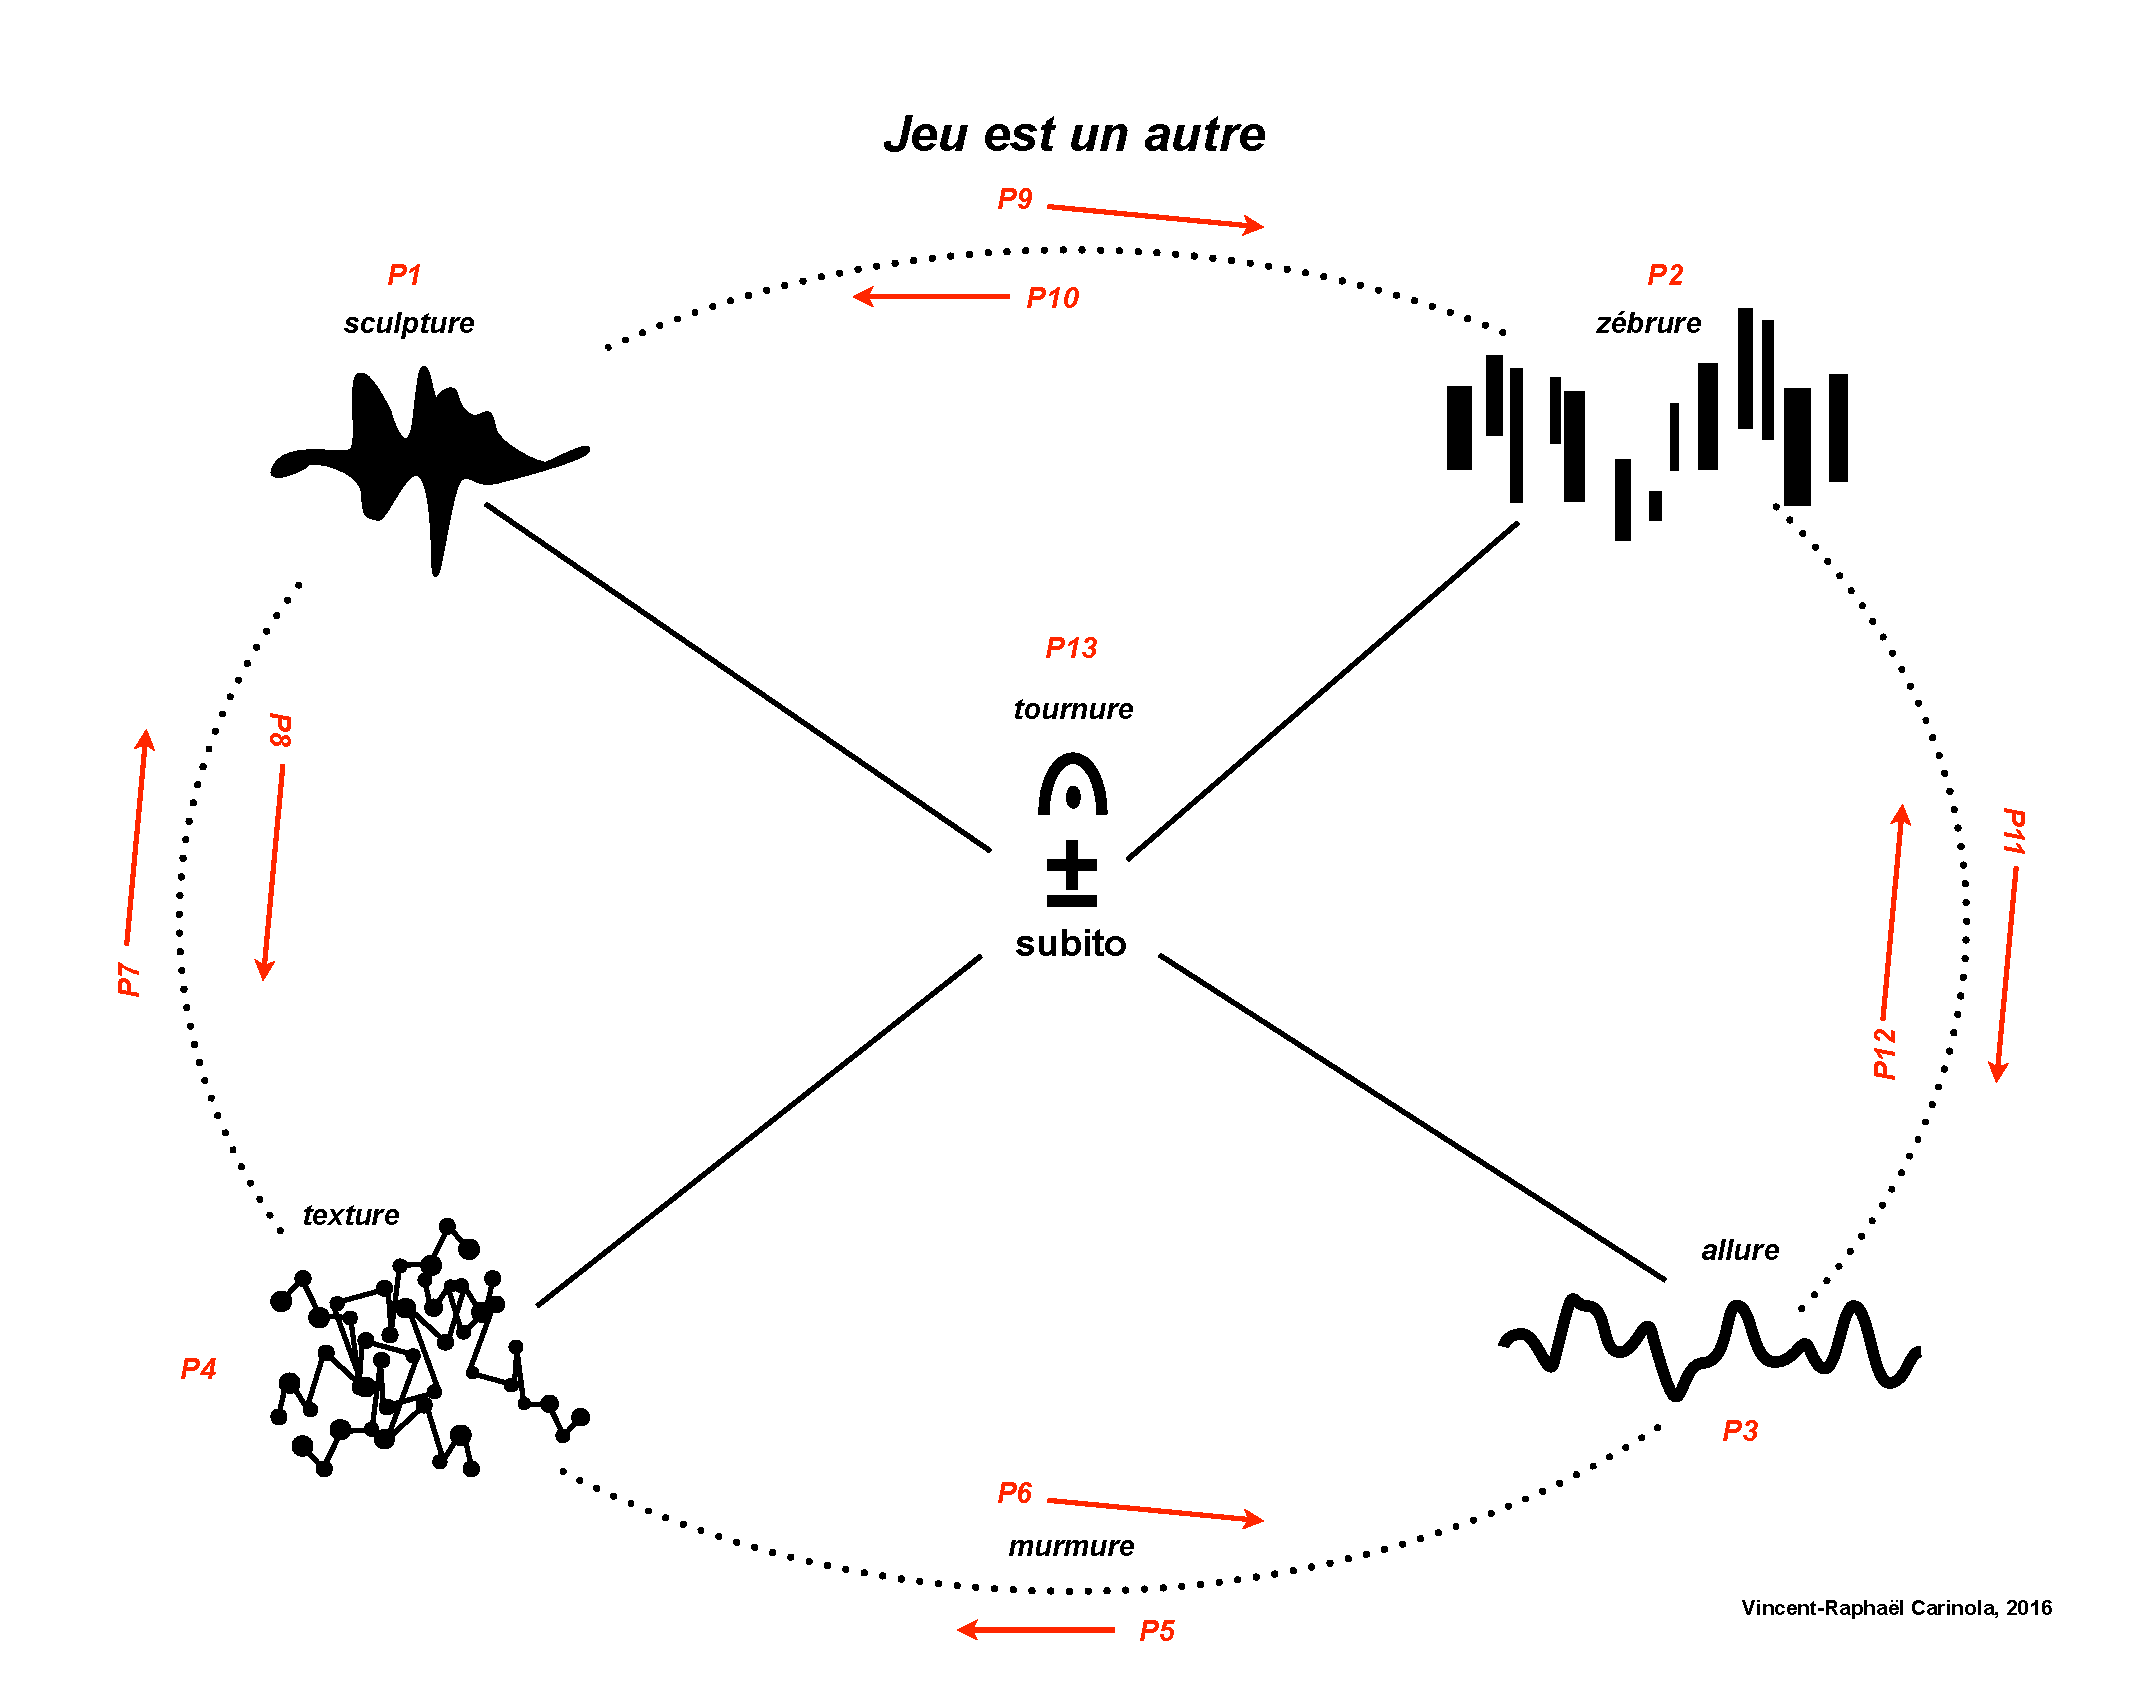
\includegraphics[width=0.8\textwidth]{imgs/jeu}
   \caption{The music score of \emph{"Jeu est un autre"} annotated (in red) with the possible \emph{ways} and \emph{stations}. The annotations are implemented as INScore's user events, they do not appear on the performer score.}
   \label{fig:sample}
\end{figure*}

%==============================================================
\section{Conclusions}
The temporal approach proposed by INScore provides an original support to dynamic music score design. It allows to express arbitrary behaviors in both musical and event times.
However, it remains limited: unlike environments such as Antescofo for example, events do not have a temporal dimension, which prevents them from being composed with logical operations. It would also be interesting to extend the temporal dimensions of an object to all its graphic attributes, so that its displacements in time could be translated into the graphical space by the variation of its attributes.

%\begin{acknowledgments}
%At the end of the Conclusions, acknowledgements to people, projects, funding agencies, etc. can be included after the second-level heading ``Acknowledgments'' (with no numbering).
%\end{acknowledgments} 

%%%%%%%%%%%%%%%%%%%%%%%%%%%%%%%%%%%%%%%%%%%%%%%%%%%%%%%%%%%%%%%%%%%%%%%%%%%%%
%bibliography here
\balance
%\bibliographystyle{IEEEtran}
\bibliography{../interlude}



\end{document}
